%!TEX root=../protocol.tex	% Optional

\section{Implementierungsumgebung}

Als Implementierungsumgebung wurde die Universelle Windows-Plattform (UWP) gewählt, um den Einblick in eine neue Umgebung zu bekommen.

\subsection{UWP}

Die UWP bietet die Möglichkeit eine Anwendung nur einmal zu entwickeln und auf allen Windows Geräten auszuführen. Dadurch kann die, in dieser Übung, entwickelte App auf vielen unterschiedlichen Geräten verwendet werden, unter anderem auf mobilen Geräten, wie Smartphones und Tablets, auf PCs, HoloLens und viele weitere. Im Fall dieser Übung wurde die Anwendung aber nur mit PCs und mobilen Geräten getestet.
\\\\
Um diese Universellen Apps zu ermöglichen, bietet UWP die selbe Kern-API auf allen Geräten an. Dadurch kann auch ein App Store als einheitliche Vertriebsplattform auf unterschiedliche Geräteformen verwendet werden.

\begin{figure}[H]
	\centering
	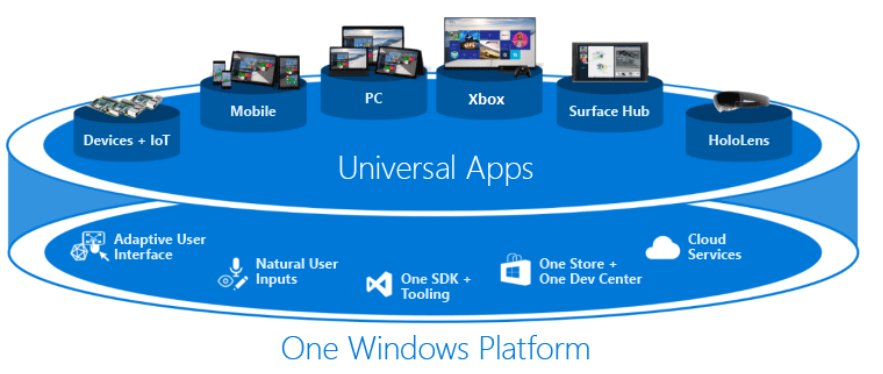
\includegraphics[width=0.7\linewidth]{images/screenshot001}
	\caption{Darstellung der UWP}
	\label{fig:screenshot001}
\end{figure}

Dennoch kann für jedes Gerät spezieller Code geschrieben werden sodass die Anwendung ein unterschiedliche Verhalten je nach Gerät aufweist. Außerdem bietet UWP universelle Steuerelemente, womit eine Benutzeroberfläche entwickelt werden kann, welche sich an die Auflösung, DPI-Dichte, Eingabeart von Geräten anpasst.
\\\\
UWP ermöglicht das Entwickeln mittels Visual C++, C\#, Visual Basic und JavaScript, wobei mit den Programmiersprachen Visual C++, C\# und Visual Basic XAML verwendet werden kann um die Benutzeroberfläche zu definieren. \cite{UWPAllgemein}
\\\\
XAML (Extensible Application Markup Language) sind XML Dateien, welche XAML Objekte initialisieren und Eigenschaften von diesen Objekten festlegen. Hierfür gibt es einen eigene XAML-Namespaces, welche festlegen, wie die Datei interpretiert wird. \cite{xamlOverview}
\\\\
Bei dieser Übung wurde C\# mit XAML zur Umsetzung der Aufgabe verwendet.

\subsection{Visual Studio}

Als am besten geeignetes Tool erweist sich Visual Studio, welches eine optimale Unterstützung für die Entwicklung von UWP Apps bietet. Bei dieser Übung wurde Visual Studio 2017 Enterprise Edition verwendet, wobei darauf zu achten ist, dass zur Verwendung von Emulatoren für andere Geräte, wie zum Beispiel Smartphones, HoloLens, ... , Visual Studio 2015 installiert sein muss. Zwar können die Emulatoren für Visual Studio 2017 gedownloadet werden, diese werden aber im Editor dann nicht angezeigt, wenn Visual Studio 2015 nicht installiert ist.
\\\\
Im Visual Studio Installer kann im Reiter ''Einzelne Komponenten'' Emulatoren für die gewünschte Windows 10 Version gedownloadet werden.

\begin{figure}[H]
	\centering
	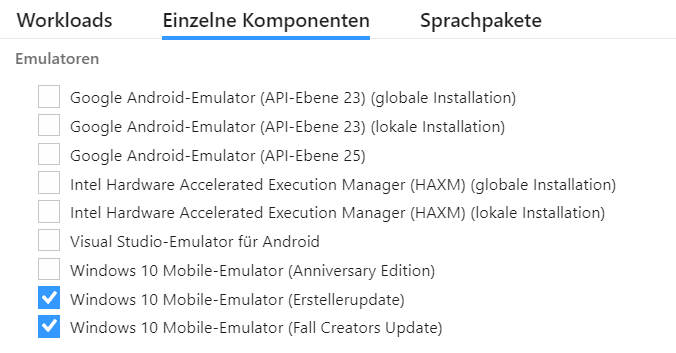
\includegraphics[width=0.7\linewidth]{images/screenshot002}
	\caption{Installieren von Emulatoren}
	\label{fig:screenshot002}
\end{figure}

In Visual Studio kann anschließend die App auf den gewünschten Gerät ausgeführt werden.

\section{REST - Schnittstelle}

Als REST - Schnittstelle wurde die entwickelte Anwendung für die Übung GK9.3 verwendet. Diese wurde nur leicht angepasst, sodass JSON Objekte gesendet werden.

\subsection{Deployen}

Die Anwendung ist im Unterverzeichnis "Cloud-Datenmanagement-Json" zu finden. Diese kann einfach deployed werden, da es sich um ein mit Maven erstelltes Programm handelt.
\\\\
Mittels folgendem Befehl wird die Anwendung auf den Port 8080 lokal gestartet.

\begin{code}{bash}
	mvn tomcat7:run-war
\end{code}

Für diese Übung wurde das Projekt auf einem Server, welcher unter der IP-Adresse 37.252.185.24 erreichbar ist, aufgesetzt.

\subsection{Verwendung}

Die REST-Schnittstelle bietet 3 Funktionen, das Anmelden eines neuen Benutzers, den Login mit einem bestehenden Account und das Löschen eines Benutzerkontos.

Bei der Registrierung muss der Vorname, der Nachname, die E-Mail-Adresse, ein Passwort sowie eine Passwort Wiederholung eingegeben werden. Diese Eingaben werden als Parameter an die Schnittstelle gesendet, nachfolgend ist ein Beispielaufruf zu sehen:

\begin{code}{bash}
	http://37.252.185.24:8080/ertl/register?vname=Marvin&nname=Ertl&email=mertl@student.tgm.ac.at&pw=abc123&pwagain=abc123
\end{code}

Die Schnittstellen für das Löschen und Einloggen von Benutzer ist ähnlich aufgebaut, beim Einloggen muss die E-Mail sowie das Passwort als Parameter mitgesendet werden und beim Löschen muss die E-Mail-Adresse mitgesendet werden.
\\\\
Die Rückgabe ist dabei immer ein JSON Objekt, welches aus einem Array mit 2 Werten besteht. Der erste Wert gibt an, ob der Befehl erfolgreich (success) oder nicht erfolgreich (error) war. Der zweite Wert gibt bei einem success weitere Informationen mit, bei einem error wird die Fehlermeldung mitgeliefert.
\\\\
Nachfolgend ist das Antwort JSON, welches bei einer erfolgreichen Registrierung zurückgeliefert wird.

\begin{code}{json}
	["success","Marvin#Ertl#mertl@student.tgm.ac.at"]
\end{code}

\section{Mobilen Applikationen}

Zum Entwickeln der Anwendung wurde in Visual Studio ein UWP Projekt erstellt, diese beinhaltet bereits die App Klasse, welche sich um das Starten/Beenden/Pausieren der Anwendung kümmert. Diese Klasse wird allen drei weiteren Klassen übergeben. Die App besteht insgesamt aus drei Ansichten, den Register Screen, dem Login Screen und der MainPage, diese Ansichten erben alle von der Page Klasse. Erfolgreiches registrieren sowie einloggen führt zur MainPage, auf welcher der Benutzer begrüßt wird und sein Vorname, Nachname sowie seine E-Mail-Adresse anzeigt. \cite{uwptutorial}
\\\\
Dabei zu beachten ist, dass jede Ansicht 2 Dateien hat, eine XAML Datei, welche die Benutzeroberfläche definiert und einer C\# Datei, welche den User Input verwaltet sowie die Ansicht.
\\\\
Zwischen den einzelnen Ansichten wird mittels der ''Navigate'' Methode gewechselt, beim Wechsel kann man nur ein Objekt mitgeben, aus diesem Grund wurde das Objekt ''Param'' angelegt, dieses beinhaltet die Instanz der App Klasse sowie einen String. Dieser wird verwendet um die Rückmeldung von der REST-Schnittstelle an die nächste Ansicht weiterzugeben.

\begin{code}{csharp}
	public class Param
	{
		public App App { get; set; }
		public string Text { get; set; }
	}
\end{code}

Eine Page reagiert mittels der Methode ''OnNavigatedTo'' auf Parameter, welche übergeben werden. Diese Methode überschreibt dabei eine Methode aus der Page Klasse. Dies geschieht wie folgt:

\begin{code}{csharp}
protected override void OnNavigatedTo(NavigationEventArgs e)
{
	base.OnNavigatedTo(e);
	
	this.param = new Param();
	this.param.App = (App)e.Parameter;
	
}
\end{code}

\subsection{Register}

Als erstes wurde die Registrierungsansicht mittels den Designer in Visual Studio erstellt.

\begin{minipage}[h]{0.4\textwidth} 
	 Dieser erlaubt es einfach aus der Toolbox Objekte mittels Drag\&Drop eine Benutzeroberfläche zu gestalten. Wobei jederzeit zwischen den Skalierung auf unterschiedlichen Geräten gewechselt werden kann. Somit kann überprüft werden, wie die Benutzeroberfläche auf diesen Geräten ausschauen würde.
\end{minipage}
\begin{minipage}[h]{0.6\textwidth}
	\begin{figure}
		\centering
		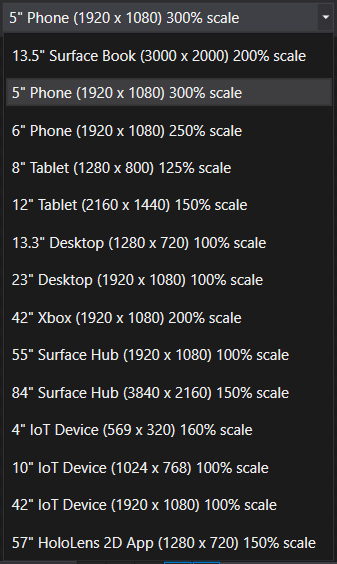
\includegraphics[width=0.45\linewidth]{images/screenshot004}
		\caption{Auswahl der Skalierung}
		\label{fig:screenshot004}
	\end{figure}
\end{minipage}


Die erstellte Oberfläche sieht im Designer wie folgt aus:

\begin{figure}[H]
	\centering
	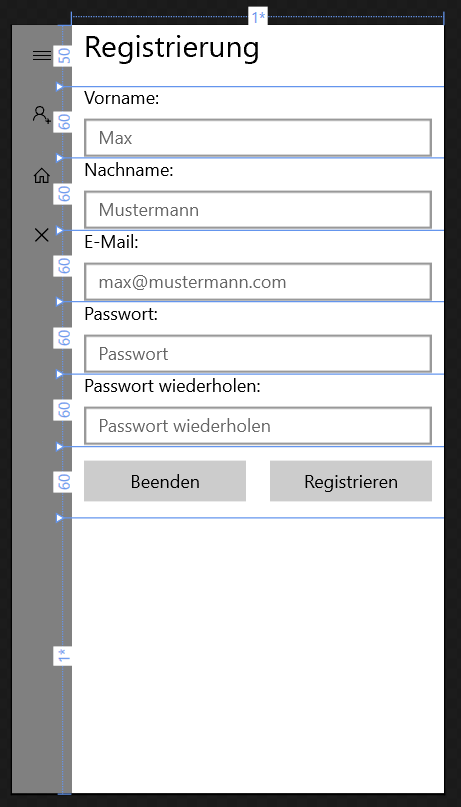
\includegraphics[width=0.4\linewidth]{images/screenshot003}
	\caption{Registrierungsoberfläche im Designer}
	\label{fig:screenshot003}
\end{figure}

Anschließend kann entweder über den Design oder direkt im XAML Code einige Änderungen vorgenommen werden. Zum Beispiel ein Event auf die Button zu legen. Nachfolgend ist ein Ausschnitt aus der XAML Datei, welcher den Button ''Registrieren'' definiert, wobei bei einem Click die Methode ''RegisterUser'' in der C\# Datei aufgerufen wird.

\begin{code}{xml}
	<Button Grid.Row="0" Grid.Column="1" Content="Registrieren" Click="RegisterUser" HorizontalAlignment="Stretch" VerticalAlignment="Stretch" Margin="10"/>
\end{code}

Die Methode, welche auf das Click Event vom Button reagiert sieht wie folgt aus:

\begin{code}{csharp}
	private async void RegisterUser(object sender, RoutedEventArgs e)
	{
		// ...
	}
\end{code}

In dieser Methode werden als erstes alle eingegebene Werte aus den Feldern ausgelesen und zu einem String zusammengesetzt, welcher die Parameter für die ''register'' Methode beinhaltet. Wobei das Passwort mittels SHA512 gehasht wird. \cite{uwphash}

\begin{code}{csharp}
	public string HashPW(string pw)
	{
		HashAlgorithmProvider objAlgProv = HashAlgorithmProvider.OpenAlgorithm(HashAlgorithmNames.Sha512);
		CryptographicHash objHash = objAlgProv.CreateHash();
		
		IBuffer buffpw = CryptographicBuffer.ConvertStringToBinary(pw, BinaryStringEncoding.Utf16BE);
		objHash.Append(buffpw);
		IBuffer buffHash = objHash.GetValueAndReset();
		
		return CryptographicBuffer.EncodeToBase64String(buffpw);
	}
\end{code}

Diese Methode erwartet einen String, dieser wird mittels SHA512 gehasht und anschließend zurückgeliefert. Dies wird bereits am Client durchgeführt, um zu verhindern, dass das Passwort während der Übertragung abgefangen wird.
\\\\
Nun wird ein Request an den Server mit den Parameter gesendet und auf eine Antwort gewartet, falls keine Verbindung mit den Server hergestellt werden kann, wird eine Fehlermeldung ausgegeben.

\begin{code}{csharp}
	string param = "vname=" + this.vname.Text + "&nname=" + this.nname.Text + "&email=" + this.email.Text + "&pw=" + this.param.App.HashPW(this.pw.Password) + "&pwagain=" + this.param.App.HashPW(this.pwagain.Password);
	
	Uri geturi = new Uri("http://37.252.185.24:8080/ertl/register?" + param);
	string response = "";
	try
	{
		System.Net.Http.HttpClient client = new System.Net.Http.HttpClient();
		System.Net.Http.HttpResponseMessage responseGet = await client.GetAsync(geturi);
		response = await responseGet.Content.ReadAsStringAsync();
	}
	catch (System.Net.Http.HttpRequestException)
	{
		this.errormessages.NavigateToString("Fehler beim Verbinden mit den Server.");
		return;
	}
\end{code}

Als Antwort wird ein JSON Objekt zurückgesendet, diese ist wie bereits oben beschrieben definiert. Zum Verarbeiten des Objektes wurde auf die Library Newtonsoft.Json zurückgegriffen, diese kann einfach mittels dem NuGet Package Manager installiert werden.
\\\\
Als erstes wird unterschieden ob es ein success oder error war, war die Registrierung erfolgreich wird der Benutzer auf die MainPage weitergeleitet.

\begin{code}{csharp}
Newtonsoft.Json.Linq.JArray result = (Newtonsoft.Json.Linq.JArray)JsonConvert.DeserializeObject(response);
if (((string)result[0]).Equals("error"))
{
	this.errormessages.NavigateToString((string)result[1]);
	return;
}
else if (((string)result[0]).Equals("success"))
{
	this.errormessages.NavigateToString(response);
	
	this.param.Text = (string)result[1];
	Frame.Navigate(typeof(MainPage), this.param);
	return;
}
\end{code}

\subsection{Login}

Beim der Login Ansicht wurde nach dem selbem Prinzip vorgegangen, nur wird beim Anmelden nur das Passwort und die E-Mail-Adresse benötigt. Wie jede Ansicht bietet auch diese ein Menü, diese kann über die drei horizontalen Balken erweitert werden, sodass neben den Buttons auch noch die Bezeichnungen stehen. Diese Button ermöglichen das Wechseln zwischen der Registrierung und dem Login, sowie einen Button zum Beenden der Anwendung. 
\\\\
Bei Fehlermeldung werden diese unterhalb der Buttons in einer WebView dargestellt. Mittels der Methode ''NavigateToString'' kann der Text in der View angezeigt werden, wobei dieser als HTML Code interpretiert wird. Dies wurde gewählt, da mehrere Fehlermeldung von Server nur mittels ''<br>'' getrennt zurückgesendet werden.

\begin{code}{csharp}
	this.errormessages.NavigateToString("Fehlermeldung");
\end{code}

Dies sieht wie folgt aus:

\begin{figure}[H]
	\centering
	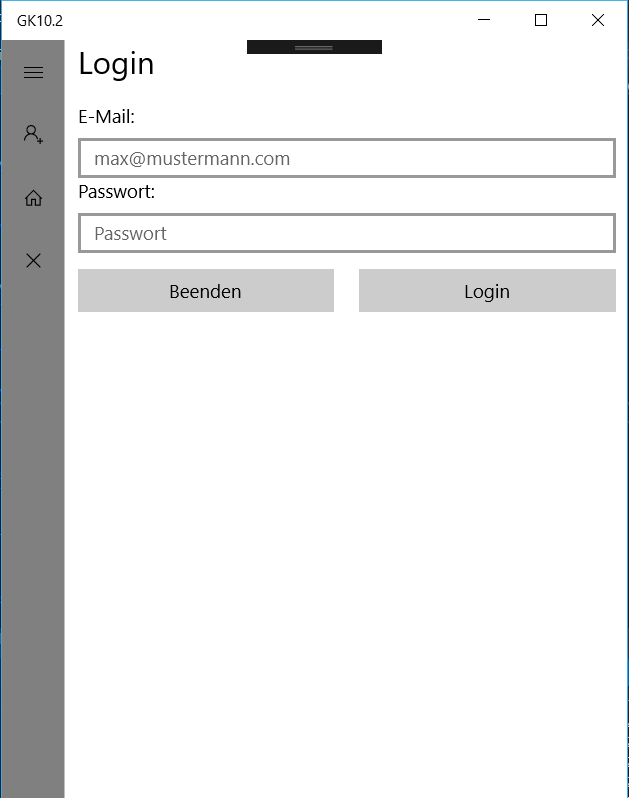
\includegraphics[width=0.5\linewidth]{images/screenshot005}
	\caption{Login Ansicht auf Windows 10}
	\label{fig:screenshot005}
\end{figure}

Ansonsten ist diese Ansicht gleich aufgebaut, bei der Anfrage an die REST-Schnittstelle wird nun nur das Passwort sowie die E-Mail-Adresse übergeben, ist das Anmelden erfolgreich wird der Benutzer zur MainPage weitergeleitet.

\begin{code}{csharp}
	string param = "email=" + this.email.Text + "&pw=" + this.param.App.HashPW(this.pw.Password);
	
	Uri geturi = new Uri("http://37.252.185.24:8080/ertl/login?" + param);
\end{code}

\subsection{Mainpage}

Ist die Ansicht, welcher der Benutzer bei einer erfolgreichen Registrierung oder Anmeldung sieht. Wurde ein Emulator und Visual Studio 2015 installiert, hat der Entwickler auch die Möglichkeit die Anwendung in einem Emulator zu starten.
\\\\
Die MainPage hat eine andere Menubar im Vergleich zum Login oder Registrieren. In dieser hat man die Möglichkeit sich abzumelden, den Account zu löschen oder die Anwendung zu beenden.
\\\\
Hierfür muss ein Request an die Methode ''delete'' gesendet werden, welche als Parameter die E-Mail-Adresse des Accountes hat.

\begin{code}{csharp}
	string param = "email=" + this.emailAdr;
	
	Uri geturi = new Uri("http://37.252.185.24:8080/ertl/delete?" + param);
\end{code}

Dies sieht dann mit einem erfolgreichen Login wie folgt aus:

\begin{figure}[H]
	\centering
	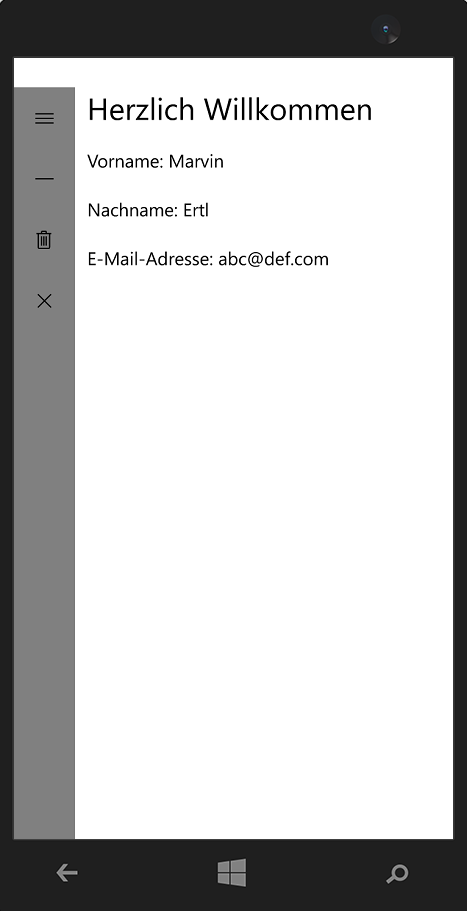
\includegraphics[width=0.4\linewidth]{images/screenshot006}
	\caption{Ausführen der Anwendung im Emulator}
	\label{fig:screenshot006}
\end{figure}


\subsection{Deployen}

Nach einigem Testen kann nun die Anwendung deployed werden, hierfür muss die App als erstes gepackt werden. Dies geschieht über einen Rechtsklick auf das Projekt in Visual Studio. Dort gibt es die Auswahlmöglichkeit ''Store'' mit den Unterpunkt ''Create App Package''. Wurde dies ausgewählt werden noch einige Informationen wie zum Beispiel Version, Name, verlangt. Anschließend kann entschieden werden, ob die App gleich direkt in den Store geladen wird, in diesem Fall wurde dies nicht gemacht.
\\\\
Abschließend muss noch die Plattform ausgewählt werden, auf welcher die App läuft für Smartphones wird ARM benötigt für Desktop x86 oder x64. Es können aber auch alle Plattformen auf einmal ausgewählt werden.
\\\\
Nun erhält man einen Ordner mit einigen Dateien, die wichtigste davon ist die Datei mit der Endung ''.appxbundle'', dabei handelt es sich um die Installationsdatei. \cite{packaging} Um die Entwicklerversion zu installieren, gibt es ein PowerShell Script, welches ausgeführt werden muss. Ansonsten kann mittels einem Doppelklick auf die Datei ''.appxbundle'' wird die Installation gestartet, dies sieht wie folgt aus: 

\begin{figure}[H]
	\centering
	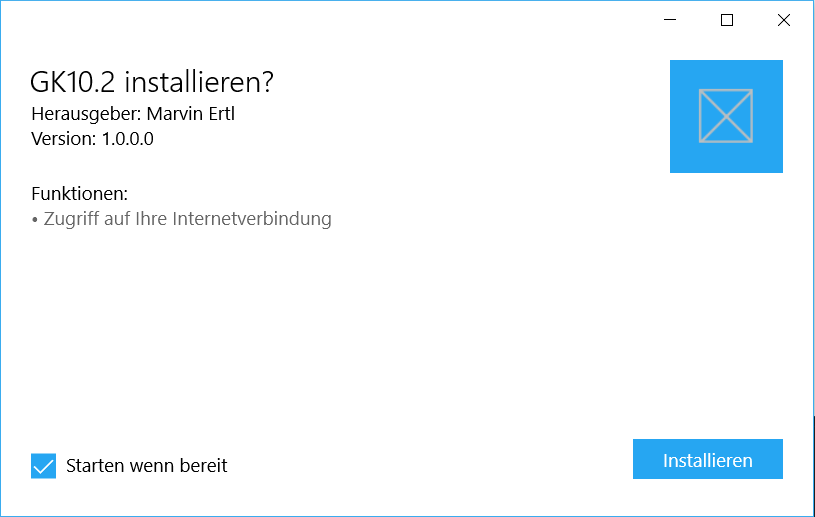
\includegraphics[width=0.7\linewidth]{images/screenshot007}
	\caption{Installieren einer App}
	\label{fig:screenshot007}
\end{figure}

Darauf zu achten ist, dass unter den Windows Einstellungen in der Kategorie ''Für Entwickler'' erlaubt wird, Apps aus anderen Quellen außer dem App-Store zu erlauben.

\section{Testen}

Um das Testen der Anwendung möglichst einfach zu machen und Regressiv zu wiederholen, wurde auf UI Automation von UWP Apps gesetzt. Dafür muss als erstes der WinAppDriver installiert werden. \cite{WinAppDriver}

\subsection{UI Automation}

Microsoft UI Automation is ein Framework um auf Elemente am Desktop zuzugreifen um die Benutzeroberfläche zu bedienen. Aus diesem Grund wurde ein zweites Projekt erstellt, welches sich um das Testen der Anwendung kümmert. Mittels diesem Framework können nicht nur eigene Anwendungen getesten werden, sondern auch Anwendungen von Drittanbieter oder Windows eigene Anwendungen. \cite{uiautooverview}
\\\\
Im Repository des Win App Drivers gibt es auch einige Beispiel, auf Basis des Beispiels für den Windows Rechner wurde eigene Testfälle entwickelt.

\subsection{Testaufbau}

Das Projekt besteht aus 2 Klassen, eine Klasse GKSession, diese startet die Anwendung und die Klasse ScenarioStandard beinhaltet die Testfälle.
\\\\
Um die Anwendung starten zu können, muss die App ID der Anwendung gefunden werden, diese kann in den App Package Informationen gefunden werden. \cite{appid} Nun kann die Anwendung wie folgt gestartet werden und eine Session erstellt werden:

\begin{code}{csharp}
                DesiredCapabilities appCapabilities = new DesiredCapabilities();
appCapabilities.SetCapability("app", AppId);
appCapabilities.SetCapability("deviceName", "WindowsPC");
session = new WindowsDriver<WindowsElement>(new Uri(WindowsApplicationDriverUrl), appCapabilities);
\end{code}

Nun kann in der Scenario Klasse Testfälle definiert werden, diese müssen mittels ''[TestMethod]'' gekennzeichnet sein. Mittels der Methode ''FindElementByName'' können nun die Buttons bzw. Eingabefelder gefunden werden und daraufgeklickt bzw. Werte eingegeben werden. Schlussendlich wird überprüft, ob nun ''Herzlich Willkommen'' in der Anwendung angezeigt wird.

\begin{code}{csharp}
	session.FindElementByName("Vorname:").Click();
	session.FindElementByName("Vorname:").SendKeys("Marvin");
	session.FindElementByName("Nachname:").Click();
	session.FindElementByName("Nachname:").SendKeys("Ertl");
	session.FindElementByName("E-Mail:").Click();
	session.FindElementByName("E-Mail:").SendKeys("abc@def.com");
	session.FindElementByName("Passwort:").Click();
	session.FindElementByName("Passwort:").SendKeys("12345");
	session.FindElementByName("Passwort wiederholen:").Click();
	session.FindElementByName("Passwort wiederholen:").SendKeys("12345");
	session.FindElementByXPath("//Button[@Name='Registrieren']").Click();
	
	Assert.AreEqual("Herzlich Willkommen", session.FindElementByName("Herzlich Willkommen").Text);
\end{code}



\begin{minipage}[h]{0.4\textwidth}
	Anschließend wurde mit einigen Testfällen überprüft ob die Anwendung richtig funktioniert bzw. ob bei einem erneuten Ausführen die Testfälle auch erfolgreich sind. Es wurde überprüft ob sich der Benutzer Registrieren/Anmelden kann und ob der Account gelöscht werden kann. Weiters wurden einige Fehlermeldungen überprüft wie zum Beispiel ein falsche Passwort, einen Benutzer mit bereits vorhanden E-Mail-Adresse registrieren. 
	\\\\ 
	Diese Test könnten nun auch mittels einem Continuous  Integration Service verbunden werden, sodass bei jedem Build automatisch diese Test ausgeführt werden. Das Ausführen der Testfälle könnte auch von einem anderen Server aus gestreamt werden.
\end{minipage}
\begin{minipage}[h]{0.6\textwidth}
	\begin{figure}[H]
		\centering
		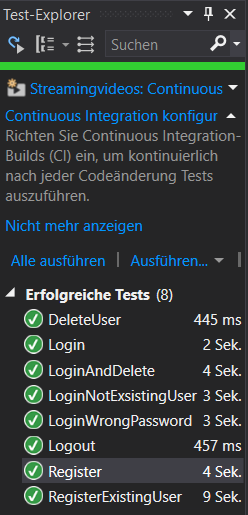
\includegraphics[width=0.5\linewidth]{images/screenshot008}
		\caption{Test Explorer in Visual Studio}
		\label{fig:screenshot008}
	\end{figure}
\end{minipage}



